% Täällä kerrotaan aikaisemmista, vastaavista projekteista

\section{Aikaisempia opetusohjelmontikieliä}
Ohjelmoinnin opettamiseen on kehitelty
monia erilaisia ohjelmointikieliä.
Tässä luvussa esittelen muutamia
historiallisesti merkittäviä
ohjelmoinninaloituskieliä.
Lisäksi esittelen myös muutamia uusia
ohjelmointikieliä, jotka toimivat
EppaBasicin tavoin selainympäristössä.

Ensimmäisillä ohjelmointikielillä
ei useinkaan voinut tehdä graafisia
ohjelmia, sillä tietokoneiden
laitteisto tuki harvoin
muita kuin tekstipohjaisia
käyttöliittymiä.
Moniin näistä kielistä
on myöhemmin lisätty
grafiikkaominaisuuksia laitteiston
kehittymisen myötä.

Yksi ensimmäisistä ohjelmoinnin
opettamiseen kehitetyistä
ohjelmointikielistä oli
Dartmouth Collegessa vuonna 1964
kehitetty BASIC \cite{basic}.
BASIC kehitettiin erityisesti
opiskelijoille, joilla ei ollut
tietojenkäsittelytieteellistä
taustaa \cite{language_history}.
Alkuperäinen BASIC oli hyvin
rajoittunut, mutta myöhemmät
murteet ovat tuoneet mukanaan
kieleen uusia ominaisuuksia.
Eräs merkittävimmistä
BASIC-murteista on
Microsoftin kehittämä
Visual Basic \cite{vb.net}.
Toisaalta myös suomalaisen
Jukka Lavosen kehittämä
CoolBasic \cite{cb} on ollut merkittävä
EppaBasicin kannalta, sillä
se on inspiroinut EppaBasicin
kehitystyötä.

Ohjelmointikielet, jotka ovat
toistensa murteita,
muistuttavat rakenteeltaan
toisiaan.
Murteet eivät välttämättä
ole yhteensopivia keskenään,
joten niitä voidaan kutsua
myös omiksi kielikseen.
Tästä syystä murteilla
usein onkin omat nimensä.

Yksi ensimmäisistä ohjelmointikielistä,
jolla pystyi tekemään grafiikkaa,
oli vuonna 1967 kehitetty Logo.
Se muistetaan erityisesti
kilpikonna-grafiikastaan,
jossa ohjelmakomennoilla
siirretään kilpikonnaa,
joka piirtää kulkiessaan
näytölle viivan.
Logo on saanut vaikutteita vuonna 1958
julkaistusta Lisp-ohjelmointikielestä.

Vuonna 1970 Niklaus Wirth
julkaisi Pascal-ohjelmointikielen
\cite{pascal}.
Kieli suunniteltiin erityisesti
opetuskäyttöön, ja se yhdisti
aikansa yleisimpien ohjelmointikielten
parhaiksi katsottuja ominaisuuksia
\cite{language_history}.
Pascal oli yritysten käytössä aina
1990-luvulle asti, kunnes muut kielet
syrjäyttivät sen.

2000-luvulle tultaessa alkoi
verkkoselainten kehittyessä
ilmestyä ohjelmointikieliä
myös selainympäristöön.
Tällaisille kielille on tyypillistä,
että niillä voi helposti luoda
ainakin yksinkertaista grafiikkaa.

Eräs selainympäristössä toimiva
ohjelmointikieli on
MIT:n kehittämä
Scratch-ohjelmoin\-ti\-kieli
\cite{scratch}
(ks. Kuva \ref{img:scratch}).
Scratch on visuaalinen ohjelmointikieli,
mikä tarkoittaa sitä, että
kieltä ohjelmoidaan raahaamalla
hiirellä komentopalikoita
ohjelmointialueelle.
Komentopalikoiden avulla
voi liikuttaa ja pyörittää
kuvia.

\begin{figure}[h]
    \centering
    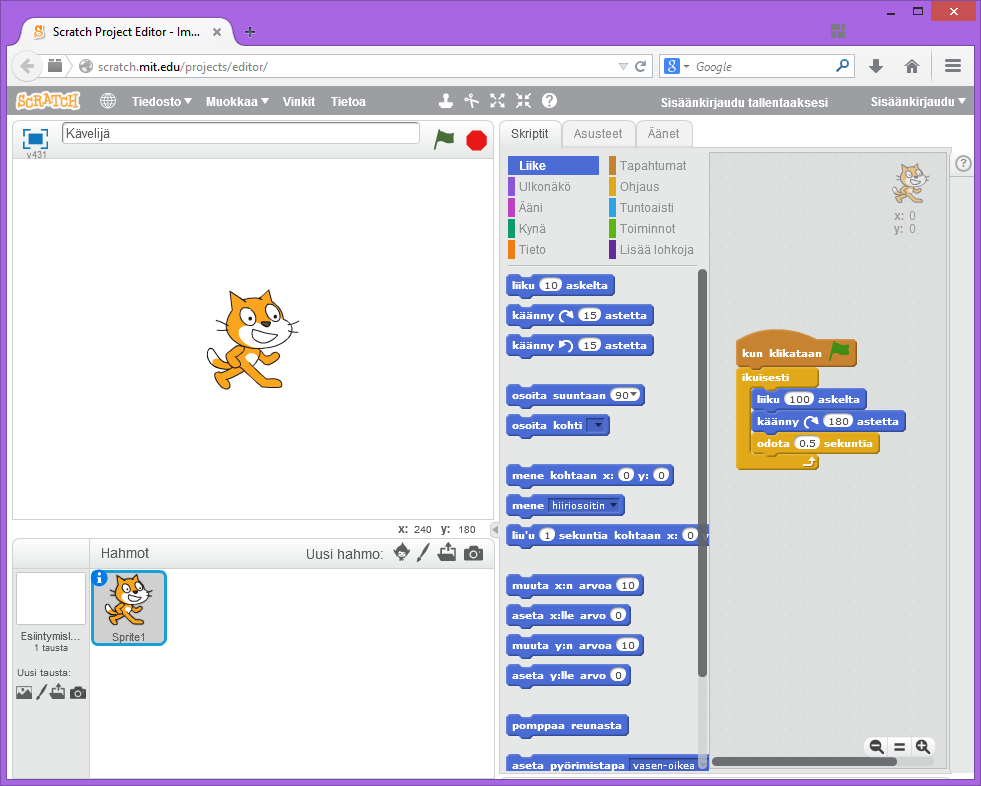
\includegraphics[width=1\textwidth]{scratch}
    \caption{Scratch-ohjelmointiympäristö, jossa vasemmassa yläkulmassa suoritusalue ja oikealla ohjelmointialue, jossa lyhyt ohjelmakoodi.}
    \label{img:scratch}
\end{figure}


OPS 2016 -opetussuunnitelman
toteuttamisessa mukana olleen
opetusneuvos Leo Pahkinin mukaan
ala-asteella on tarkoitus tutustua
visuaalisiin ohjelmointikieliin
\cite{koodi2016_ops}.
Yläasteella hänen mukaansa
on tarkoitus tutustua
ohjelmointikieliin, joita
ohjelmoidaan kirjoittamalla koodia.

EppaBasicin on tarkoitus olla
yksi mahdollisuus yläluokilla
käytettäväksi ohjelmointikieleksi.
Myös käytön alaluokilla on
mahdollista.